\documentclass{article}

\usepackage[utf8]{inputenc}
\usepackage[a4paper, total={6in, 8in}]{geometry}
\usepackage{amsmath}
\usepackage{amssymb}
\usepackage{pgfplots}
\usepackage{array}
\usepackage{enumitem}
\usepackage[scr=boondoxo,scrscaled=1.05]{mathalfa}
\usepackage{xfrac}

\pgfplotsset{compat = 1.18}
\definecolor{blue}{RGB}{31,18,213}
\definecolor{green}{RGB}{31,182,83}
\definecolor{purple}{RGB}{158, 86, 209}

\setlength\parindent{0pt}

\newcommand{\eqname}[1]{\tag*{#1}}
\newcommand{\work}{\mathscr{L}}
\newcommand{\Def}[1]{\setlength\parindent{0pt}\underline{\textit{Def.}} \emph{#1}:}


\title{Formulario Fisica (Seconda Parte)}
\author{Edoardo Figini}
\date{aa 2021-2022}

\begin{document}

\maketitle

\tableofcontents
\newpage

\section{Dinamica di sistemi di oggetti}

\subsection{Equazioni cardinali della dinamica dei sistemi}

\begin{equation}
    \boxed{\vec{R}^{(e)} = \frac{d\vec{Q}}{dt}}
\end{equation}
\begin{equation}
    \boxed{\frac{d\vec{L}_{TOT}}{dt} = \vec{M}_{TOT}{^{(e)}}}
\end{equation}

\subsection{Urti - fenomeni d'urto tra due oggetti}
$\vec{Q}$ è costante durante l'urto
\subsubsection{Tipologie di urti}
\begin{itemize}
    \item   \textbf{Urti elastici} \\
            $K_{TOT}$ si conserva:
            \begin{equation*}
                \frac{1}{2}m_1v_1^{\tiny{(-)}^2} + 
                \frac{1}{2}m_2v_2^{\tiny{(-)}^2} = 
                \frac{1}{2}m_1v_1^{\tiny{(+)}^2} + 
                \frac{1}{2}m_2v_2^{\tiny{(+)}^2} 
            \end{equation*}
            $\to$ risolvibile solo in una dimensione
    \item   \textbf{Urti anleastici}
    
            \begin{equation*}
                K_{TOT}^{\tiny{(-)}} \neq K_{TOT}^{\tiny{(+)}}
            \end{equation*}
            $\to$ energia viene dispersa
    \item   \textbf{Urti perfettamente anelastici} \\
            I due oggetti si fondono in uno solo
            \begin{equation*}
                V^{\tiny{(+)}} = \frac{m_1v_1^{\tiny{(-)}} + m_2v_2^{\tiny{(-)}}}{m_1 + m_2}
            \end{equation*}
\end{itemize}


\subsection{Centro di massa}
La posizione del centro di massa è data dalla media pesata delle posizioni di ogni punto rispetto alla massa:
\begin{equation}
    \vec{r}_{\tiny{CM}} = \frac{\sum_{i=1}^N m_i \vec{r_i}}{\sum_{i=1}^N m_i}
\end{equation}

chiamando $\sum_{i=1}^N m_i$ $M$:
\begin{equation}
    \begin{cases}
        \vec{Q}=M\frac{d\vec{r}_{CM}}{dt} \\
        \vec{V}_{\tiny{CM}}=\frac{d\vec{r}_{CM}}{dt}
    \end{cases}
    \label{q e v}
\end{equation}
\begin{equation}
    \begin{cases}
        \frac{d\vec{Q}}{dt}=M\frac{d\vec{V}_{CM}}{dt} \\
        \vec{a}_{\tiny{CM}}=\frac{d^2\vec{r}_{CM}}{dt^2}
    \end{cases} 
    \label{dq e a}
\end{equation}

Ogni corpo può essere quindi studiato nel suo Centro di Massa, infatti da \eqref{q e v} e \eqref{dq e a}:
\begin{equation}
    \boxed{\vec{Q} = M\vec{V}_{\tiny{CM}}}
\end{equation}
\begin{equation}
    \boxed{\vec{R}^{(e)} = M\vec{a}_{\tiny{CM}}}
\end{equation}

Per un sistema isolato:
\begin{itemize}
    \item $\vec{R}^{(e)} = 0$
    \item $\vec{v}_{\tiny{CM}}$ costante
    \item $\vec{a}_{\tiny{CM}}$ costante
\end{itemize}

\subsection{Teoremi di König}
\begin{equation}
    \boxed{\vec{L}_{TOT_{(O)}} = \vec{r}_{CM} \times M \vec{v}_{CM} + \vec{L}_{TOT_{CM}}}
    \label{konig1}
\end{equation}
\vspace{\baselineskip}
\begin{equation*}
    K_{TOT} = \frac{1}{2}M_{TOT} \vec{V}_{\tiny{CM}}{^2} + \sum_{i=1}^N \frac{1}{2} m_i v_i{'}^2 
\end{equation*}
\begin{equation}
    \boxed{K_{TOT} = \frac{1}{2}M_{TOT} \vec{V}_{\tiny{CM}}{^2} + K_{TOT}{'}}
\end{equation}


\subsection{Lavoro ed Energia}

\begin{equation*}
    \Delta K_{TOT} = \work^{(i)}_{{i} \to {f}} + \work^{(e)}_{{i} \to {f}}
\end{equation*}

$V \to$ energia potenziale interna al sistema 

\begin{equation*}
    \work^{(i)}_{{i} \to {f}} = \work^{(inc)}_{{i} \to f} - \Delta V^{(i)}
\end{equation*}

\begin{equation*}
    \work^{(e)}_{{i} \to {f}} = \work^{(enc)}_{{i} \to f} - \Delta V^{(e)}
\end{equation*}
\vspace{\baselineskip}
\begin{equation*}
    E_m = K_{TOT} + V^{(i)} + V^{(e)}
\end{equation*}

\begin{equation*}
    \Delta E_m = \work^{(inc)}_{{i} \to {f}} + \work^{(enc)}_{{i} \to {f}}
\end{equation*}


In assenza di forze non conservative
\begin{equation*}
    \Delta E_m = 0
\end{equation*}

\vspace{\baselineskip}

\begin{equation*}
    K_{TOT} = K_{CM} + K_{TOT}{'}
\end{equation*}

\begin{equation*}
    K_{CM} + K_{TOT}{'} + \Delta V^{(i)} = \work^{(e)}_{i \to f}
\end{equation*}

Introducendo l'energia interna del sistema $U=K_{TOT}{'} + \Delta V^{(i)}$
\begin{equation}
    \Delta K_{CM} + \Delta U = \work^{(e)}_{i \to f}
\end{equation}

\vspace{\baselineskip}
\section{Sistemi Rigidi (Corpo Rigido)}
La distanza tra due oggetti puntiformni qualsiasi del sistema rimane costante nel tempo

\begin{equation*}
    \vec{v} = \vec{V_{(O')}} + \omega \times (\vec{r} - \vec{R_{(O')}})
\end{equation*}

\begin{equation}
    \vec{v_P} = \vec{V}_{CM} + \omega \times (\vec{r_P} - \vec{r}_ {CM})
\end{equation}

\begin{itemize}
    \item   Se $O'$ è in quiete rispetto a O
            \begin{equation*}
                \vec{V}_{(O')} = 0
            \end{equation*}
            \begin{equation}
                \frac{d\vec{L}_{TOT_{(O')}}}{dt} = \vec{M}_{(O')}^{(e)}
            \end{equation}
    \item   Se $O' \equiv CM$  
            \begin{equation*}
                \vec{V}_{(O')} = \vec{V}_{CM} \;\; \to \;\; \vec{V}_{(O')} \times M \vec{V}_{CM} = 0
            \end{equation*}
            \begin{equation*}
                \frac{d\vec{L}_{TOT_{CM}}}{dt} = \vec{M}_{CM}^{(e)}
            \end{equation*}
            
            \begin{equation*}
                \vec{L}_{TOT_{CM}} = \vec{L}_{TOT_{(O')}} - \vec{r}_{CM} \times M \vec{v}_{CM}
            \end{equation*}
            \begin{equation}
                \vec{L}_{TOT_{(O)}} = \vec{r}_{CM} \times M \vec{v}_{CM} + \vec{L}_{TOT_{CM}}
            \end{equation}
            I teorema di König \eqref{konig1}
\end{itemize}

\subsection{Momento di Inerzia}
Chiamando $r_i$ la distanza del punto $m_i$ dall'asse di rotazione e $\rho$ la densità:
\begin{equation}
    I = \sum_{i=1}^{N} m_i r_i^2
    \label{inerzia}
\end{equation}
\begin{equation}
    \rho(P) = \frac{dm}{dV}
    \label{densita}
\end{equation}

Da \eqref{inerzia} e \eqref{densita}:
\begin{equation*}
    I = \lim_{\Delta V \to 0} \sum_{i=1}^{N} \Delta m_i r_i^2
\end{equation*}
\begin{equation}
    \boxed{I = \iiint r^2 \rho dV} 
\end{equation}

\subsubsection{Teorema di Huygens-Steiner}
Per trovare $I$ su un asse parallelo:
\begin{equation}
    \boxed{I = T_{CM} + M d^2}
    \label{teoHS}
\end{equation}
dove $d$ è la distanza tra i due assi


\subsection{Sistemi rigidi in moto}
\subsubsection{Moto di pura traslazione}
\begin{equation*}
    \vec{Q} = M \vec{V}_{CM}
\end{equation*}
\begin{equation}
    \vec{L}_{TOT_{(O)}} = \vec{r}_{CM} \times \vec{Q}
\end{equation}
\subsubsection{Moto di pura rotazione}
$\vec{r_i}$ scomposto in componenti: 
\begin{itemize}
    \item $z_i \vec{u_z}$ lungo asse $z$
    \item $\rho_i$ perpendicolarmente a $z$
\end{itemize}
\begin{equation}
    \vec{L}_{TOT_{(O)}} = I \vec{\omega} - \sum_{i=1}^{N} m_i z_i \omega \vec{\rho_i}
\end{equation}
Se asse di rotazione è anche asse di simmetria:
\begin{equation}
    \boxed{\vec{L}_{TOT_{(O)}} = I \vec{\omega}}
\end{equation}

considerata $\vec{M_z}$ la proiezione di $\vec{M}_{(O)}^{(e)}$ lungo $z$:
\begin{equation}
        \boxed{\vec{M}_z^{(e)} = I \vec{\alpha}}
\end{equation}

\subsubsection{Moto di rotolamento}
Moto studiato nel punto di contatto del sistema con il suolo $Q$, chiamato \emph{centro di istantanea rotazione}

\begin{equation}
    \vec{v} = \vec{\omega} \times \vec{r}
\end{equation}

\begin{equation}
    |\vec{v}_{CM}| =\omega R
    \label{velocitarotolamento}
\end{equation}

da \eqref{velocitarotolamento}:

\begin{equation}
    |\vec{Q}| = M R \omega
\end{equation}

\subsection{Statica di corpi rigidi}
Condizioni necessarie per la quiete:

\begin{equation*}
    R^{(e)} = 0
\end{equation*}

\begin{equation*}
    M^{(e)}_{TOT_{(O')}}= 0
\end{equation*}

\subsection{Energia Cinetica e Lavoro delle Forze esterne}

\begin{equation}
    \boxed{K_{TOT} = \frac{1}{2} M \vec{v}_{CM}{^2} + \frac{1}{2} I \omega^2}
\end{equation}

\vspace{\baselineskip}

\begin{equation*}
    \work_{i \to f}^{(e)} = \underset{\gamma_{CM}}{\int_{A_{CM}}^{B_{CM}}}\vec{R}^{(e)} d\vec{r}_{CM} + \int_{\theta_{B}}^{\theta_{A}}\vec{M}_z^{(e)} d\theta = \Delta K_{TOT}
\end{equation*}

\begin{equation}
    \boxed{\work_{i \to f}^{(e)} = \Delta K_{CM} + \Delta K_{ROT} = \Delta K_{TOT}}
\end{equation}

\vspace{\baselineskip}
\section{Fluidi}
\Def{Fluido Ideale} non ha viscosità
\vspace{\baselineskip}

\Def{Pressione} 
    \begin{equation*}
        p = \lim_{S \to 0} \frac{F_\perp}{S} = \frac{dF_\perp}{dS}
    \end{equation*}
\begin{itemize}
    \item unità di misura nel SI
    \begin{equation*}
        p \to [Pa] = \left ( \frac{N}{m^2} \right )
    \end{equation*}
    
    \item Altre unità di misura
    \[
        [bar] \to 1 bar = 10^5 Pa 
    \]
    \[
        [atm] \to 1 atm \simeq 1,013 bar \simeq 101300 Pa
    \]
\end{itemize}

\Def{Isotropia della Pressione} La pressione non dipende dall'orientazione del sistema
\vspace{\baselineskip}

\Def{Densità} 
    \begin{equation*}
        \rho = \lim_{\Delta V \to 0} \frac{\Delta m}{\Delta V} = \frac{dm}{dV}
    \end{equation*}

\setlength\parindent{25pt} in generale:
    \begin{equation*}
        \rho = \rho(T, p)
    \end{equation*}
    
\Def{Fluidi perfetti} $\rho$ è costante $\to$ \textbf{incomprimibili} e \textbf{indilatabili}

\setlength\parindent{90pt} $\rho$ non dipende da $T$ o $p$

\Def{Forze di volume} Forze che agiscono sul volume (es. Forza peso)
\[
\vec{f_v} = \frac{\vec{F_v}}{m} \;\; \to \;\; \left [ \frac{N}{kg} \right]
\]

\Def{Equilibrio statico}
\[
\sum F = 0 \;\; \to \;\; \vec{F_v} + \vec{F_s} = 0
\]

\begin{center}$\vec{F_s} \to$ forze di superficie \end{center}

\subsection{Equazione della Statica dei fluidi}
\begin{equation}
    \boxed{\vec{\nabla} p = \vec{f_v} \cdot \rho}
\end{equation}

\begin{itemize}
    \item Se $\nexists \; \vec{f_v}$, allora $\vec{\nabla{p}}=0$, quindi $p$ è omogenea
    \item Se $\exists \; \vec{f_v}$, allora $\vec{\nabla{p}}\neq0$ e punta verso $\vec{f_v}$
\end{itemize}

\subsection{Legge di Stevino}
La pressione varia in base alla quota:
\begin{equation}
    \boxed{p = p_0 +  \rho gh}
\end{equation}

dove $\rho gh$ è detta \emph{pressione idrostatica}.

\Def{Legge di Pascal} Variazione di pressione in un punto di un liquido si trasmette inalterata a tutti i punti del liquido

\subsection{Principio di Archimede}
Ogni corpo immerso in un fluido subisce una forza diretta dal basso verso l'alto di intensità equivalente alla forza peso del volume di fluido spostato.

\begin{equation}
    \boxed{F_A = - \rho g V_f}
\end{equation}

\section{Termodinamica}

\Def{Sistema Aperto} sia scambi di calore sia di lavoro
\vspace{\baselineskip}

\Def{Sistema Chiuso} solo scambi di calore
\vspace{\baselineskip}

\Def{Sistema Isolate} non avvengono scambi
\vspace{\baselineskip}

\Def{Regola fasi di Gibbs}
\begin{equation}
N = C + 2 -F
\end{equation}

dove 
\begin{itemize}
    \item $N$ è il numero di coordinate indipendenti
    \item $C$ è il numero di specie chimiche
    \item $F$ è il numero di fasi
\end{itemize}

\vspace{\baselineskip}
\Def{Equilibrio Termodinamico}
\begin{itemize}
    \item \Def{Eq. meccanico} equilibrio delle forze e dei momenti
    \item (\emph{Eq. chimico}) 
    \item \Def{Eq. termico} i due sistemi hanno le stesse coordinate termodianmiche
\end{itemize}

\Def{Trasformazioni} evoluzione di un sistema termodinamico
\begin{center}
    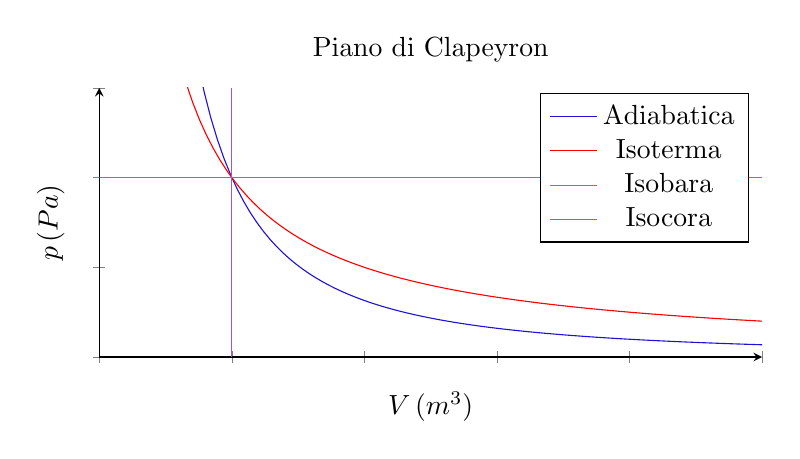
\begin{tikzpicture}
    
        \begin{axis}[
            title = Piano di Clapeyron,
            axis lines = left,
            xlabel = $V \, (m^3)$,
            ylabel = {$p \, (Pa) $},
            width= 10cm,
            height=5cm,
            ymax = 1.5,
            yticklabel=\empty,
            xticklabel = \empty
        ]
        
        \addplot [
            domain= .1:5, 
            samples=100, 
            color = blue,
        ]
        {pow(x, -(5/3))};
        \addlegendentry{Adiabatica}
        
        \addplot [
            domain= 0:5, 
            samples=100, 
            color = red,
        ]
        {1/x};
        \addlegendentry{Isoterma}
        
        
        \addplot [
            domain= 0:5, 
            samples=100, 
            color = green,
        ]
        {1};
        \addlegendentry{Isobara}
        
        \addplot[
            samples=1, 
            smooth,
            domain=0:1,
            color = purple,
        ] coordinates {(1,0)(1,1.5)};
        \addlegendentry{Isocora}
        
        
        \end{axis}
    \end{tikzpicture}
\end{center}

\subsection{Principio 0 della Termodinamica}
\Def{} Due sistemi in equilibrio termico con un terzo sono in eqilibrio tra di loro

\subsection{Equazione di stato dei gas perfetti}

\Def{Legge di Boyle}
\begin{equation}
    V \propto \frac{1}{p} \;\; (T= cost, n=cost)
\end{equation}

\vspace{\baselineskip}
\Def{Legge di Charles/ I legge di Gay-Lussac}
\begin{equation}
    V = V_0 (1+\alpha t)
\end{equation}
\[
    V \propto T \;\; (p= cost, n=cost)
\]

\vspace{\baselineskip}
\Def{(II) Legge di Gay-Lussac}
\begin{equation}
    p = p_0 (1+\alpha t)
\end{equation}

\vspace{\baselineskip}
\Def{Legge di Avogadro} Volumi uguali di gas diversi nelle stesse condizioni di temperatura contengono lo stesso numero di molecole.

una mole di qualsiasi sostanza contiene sempre lo stesso numero di atomi/molecole: 
\begin{equation}
    N_A = 6.022 * 10^{23}
    \label{avo}
\end{equation}
\[
    V \propto n
\]

\Def{Equazione di stato dei gas perfetti}
\begin{equation}
    \boxed{pV = nRT}
\end{equation}

$R=8.3145 \frac{J}{mol \cdot K}$ è la costante universale dei gas
\vspace{\baselineskip}

$R=N_A + K_B$, dove $N_A$ è il \emph{Numero di Avogadro} \eqref{avo} e $K_B$ è detta \emph{costante di Boltzmann} e vale $K_B=8,3145 \frac{J}{mol \cdot K}$

\vspace{\baselineskip}
Forma differenziale:
\begin{equation}
    V dp + p dV = nR dT
\end{equation}


\vspace{\baselineskip}
\Def{Legge di Dalton per i gas ideali (Legge delle pressioni parziali)} permette di trattare miscele di gas perfetti
\begin{equation}
    \boxed{p = \sum_{i=1}^{N}\frac{n_i RT}{V}}
\end{equation}

\subsection{Lavoro}
\Def{Lavoro compiuto dal sistema} $\work > 0$, detto lavoro fatto $\work_F$

\vspace{\baselineskip}
\Def{Lavoro subito dal sistema} $\work < 0$, detto lavoro subito $\work_S$

\vspace{\baselineskip}
\Def{Lavoro compiuto dal Gas}

\begin{equation}
    \boxed{\work_{GAS} = \int p_e dV}
\end{equation}

\begin{itemize}
    \item per \emph{espansioni}: $dV > 0 \;\to\; \work > 0$
    \item per \emph{compressioni}: $dV < 0 \;\to\; \work < 0$
\end{itemize}

Casi particolari:
\begin{itemize}
    \item ambiente a pressione costante: $\work = p_e \Delta V$ 
    \item ambiente a pressione nulla (vuoto): $\work = 0$
    \item trasformazione quasi statica: $\work = \int p dv$ (equilibrio meccanico)
\end{itemize}

Trasformazioni reversibili di gas perfetti:
\begin{itemize}
    \item \emph{Isobara}: $\boxed{\work_{A \to B} = p \Delta V}$
    \item \emph{Isocora}: $\boxed{\work_{A \to B} = 0}$
    \item \emph{Isoterma}: $\boxed{\work_{A \to B} = nRT \cdot \ln{\left (\frac{V_B}{V_a} \right)}}$
\end{itemize}

\subsection{Energia interna per i gas ideali}
\Def{Energia interna} energia potenziale associata alle trasformazionio adiabatiche (funzione di stato)
\begin{equation}
    \boxed{\Delta U = m c_v \Delta T}
\end{equation}

\subsection{Primo principio della termodinamica}
\begin{equation}
    \boxed{Q= \work_{A \to B} + \Delta U}
\end{equation}

Forma differenziale:
\begin{equation}
    \boxed{\delta Q= \delta \work_{A \to B} + dU}
\end{equation}

\vspace{\baselineskip}
\Def{Capacità termica}
\[
C = \frac{\delta Q}{dT} \;\; \left( \frac{J}{K} \right)
\]

\vspace{\baselineskip}
\Def{Calore specifico}
\[
c = \frac{C}{m} \;\; \left( \frac{J}{Kg \cdot K} \right) 
\]
\[
c = \frac{C}{n} \;\; \left( \frac{J}{mol \cdot K} \right)
\]

\subsection{Calorimetria}
\Def{Calore} Energia trasferibile tra i sistemi
\begin{equation}
    \boxed{Q = m c \Delta T}
\end{equation}
Durante un cambio di fase il Calore è definito come:
\begin{equation}
    \boxed{Q = m \lambda}
\end{equation}
Dove $\lambda$ è detto \emph{calore latente} ed è specifico per ogni sostanza.

\begin{center}
    \begin{tikzpicture}
    
        \begin{axis}[
            title=Fusione,
            clip=false,
            axis lines = left,
            xlabel = $Q_{fornito}$,
            ylabel = $T$,
            xlabel style = {at={(axis description cs:1,0)},anchor=north east},
            ylabel style = {at={(axis description cs:0,1)},anchor=north east,rotate=-90},
            width= 10cm,
            height=5cm,
            ymax = 5,
            ymin = 0,
            xmax = 10,
            xmin = 0,
            ytick={2.5},
            yticklabel= $T_{fusione}$,
            xticklabel = \empty,
            ymajorgrids = true,
            grid style = dashed
        ]

        \addplot[
            domain=1:3
        ]{(1/2)*x + 1}
        node[anchor=north west, pos=0.3]{$Q=mc\Delta T$};

        \addplot[
            domain=3:6
        ]{2.5}
        node[anchor=south east, pos=0.9]{$Q=m\lambda$};

        \addplot[
            domain=6:9
        ]{(1/2)*x - .5}
        node[anchor=north west, pos=0.7]{$Q=mc\Delta T$};
        
        \end{axis}
    \end{tikzpicture}
\end{center}

\subsection{Realzione di Mayer}
\begin{equation}
    c_p = c_v + R
\end{equation}

\subsection{Trasformazioni Politropiche}
Trasformazioni notevoli reversibili

\[
pV^\alpha = cost
\]

\begin{itemize}
    \item Adiabatica: $\alpha = \gamma $
    \item Isoterma: $\alpha = 1$
    \item Isocora: $\alpha = 0$
    \item Isobara: $\alpha = \infty$
\end{itemize}

\subsubsection{Adiabatica reversibile}
\begin{equation}
    T \cdot V ^{(\gamma - 1)} = cost
\end{equation}
\begin{equation}
    p V ^{\gamma} = cost
\end{equation}

\Def{$\gamma$} $\frac{c_p}{c_v}$
\begin{center}
\begin{tabular}{| l | c | c | c |}
    \hline
    \textbf{Gas} & \textbf{$c_v$} & \textbf{$c_p$} & \textbf{$\gamma$} \\
    \hline
    Monoatomico & $\sfrac{3}{2} R$ & $\sfrac{5}{2} R$ & $\sfrac{5}{3}$\\
    Biatomico & $\sfrac{5}{2} R$ & $\sfrac{7}{2} R$ & $\sfrac{7}{5}$\\
    Poliatomico & $3 R$ & $4 R$ & $\sfrac{4}{3}$\\
    \hline
\end{tabular}
\end{center}

\begin{center}
\begin{tabular}{| c | c |}
    \hline
    \textbf{Compressione Adiabatica} & \textbf{Espansione Adiabatica} \\
    \hline
    $\work_S < 0 \to$ & $ \to \work_F > 0$ \\
    \hline
    $\Delta U > 0$ & $\Delta U < 0$\\
    $\Delta T > 0$ & $\Delta T < 0$\\
    $\Delta V < 0$ & $\Delta V > 0$\\
    $\Delta p > 0$ & $\Delta p < 0$\\
    \hline
\end{tabular}
\end{center}

\subsubsection{Isoterma Reversibile}
\begin{center}
\begin{tabular}{| c | c |}
    \hline
    \textbf{Espansione Isoterma} & \textbf{Compressione Isoterma} \\
    \hline
    $Q_A > 0 \to$ & $\to Q_C < 0$ \\
    $\to \work_F > 0$ & $ \work_S < 0 \to$ \\
    \hline
    $\Delta U = 0$ & $\Delta U = 0$\\
    $\Delta T = 0$ & $\Delta T = 0$\\
    $\Delta V > 0$ & $\Delta V < 0$\\
    $\Delta p < 0$ & $\Delta p > 0$\\
    \hline
\end{tabular}
\end{center}

\subsubsection{Isocora Reversibile}
\begin{center}
\begin{tabular}{| c | c |}
    \hline
    \textbf{Riscaldamento Isocoro} & \textbf{Raffreddamento Isocoro} \\
    \hline
    $Q_A > 0 \to$ & $\to Q_C < 0$ \\
    \hline
    $\work = 0$ & $\work = 0$ \\
    $\Delta U > 0$ & $\Delta U < 0$\\
    $\Delta T > 0$ & $\Delta T < 0$\\
    $\Delta V = 0$ & $\Delta V = 0$\\
    $\Delta p < 0$ & $\Delta p > 0$\\
    \hline
\end{tabular}
\end{center}

\subsubsection{Isobara Reversibile}
\begin{center}
\begin{tabular}{| c | c |}
    \hline
    \textbf{Espansione Isobara} & \textbf{Compressione Isobara} \\
    \hline
    $Q_A > 0 \to$ & $Q_C < 0 \to$ \\
    $\to \work_F > 0$ & $ \to\work_S < 0$ \\
    \hline
    $\Delta U > 0$ & $\Delta U < 0$\\
    $\Delta T > 0$ & $\Delta T < 0$\\
    $\Delta V > 0$ & $\Delta V < 0$\\
    $\Delta p = 0$ & $\Delta p = 0$\\
    \hline
\end{tabular}
\end{center}

\subsection{Rendimento}
\Def{Rendimento} percentuale di calore assorbito che la macchina riesce a trasformare in Lavoro netto.
\begin{equation}
    \boxed{\eta = \frac{\work}{Q_A}}
\end{equation}

\vspace{\baselineskip}
\Def{Coefficiente di prestazione (COP)} 
\begin{itemize}
    \item Per Pompa di Calore:
        \begin{equation}
            COP_C = \left | \frac{Q_C}{\work} \right |
        \end{equation}
    \item Per Frigorifero:
        \begin{equation}
            COP_F = \frac{Q_A}{|\work|}
        \end{equation}
\end{itemize}

\Def{Ciclo di Carnot} Ciclo Termodinamico \emph{Reversibile} sia termico sia frigorifero
\begin{equation}
    \eta = 1 - \frac{T_1}{T_2}
\end{equation}

\subsection{Secondo Principio daella termodinamica}
\Def{Enunciato di Kelvin-Plank} è impossibile realizzare una trasformazione il cui unico risultato sia quello di convertire completamente in lavoro il calore assorbito dal sistema termodinamico

\vspace{\baselineskip}
\Def{Enunciato di Clausius} è impossibile realizzare una trasformazione il cui unico risultato sia quello di trasferire (spontaneamente) calore da un corpo freddo a uno caldo

\vspace{\baselineskip}
\Def{Teorema di Carnot} date due sorgenti $T_1$ e $T_2 > T_1$
\begin{itemize}[leftmargin={130pt}]
    \item tutte le macchine reversibili operanti tra queste due sorgenti hanno lo stesso rendimento 
    \[
    \eta_{REV} = \left ( 1 - \frac{T_2}{T_1} \right )
    \]
    \item le macchine irreversibili che operano tra queste due sorgenti hanno rendimento
    \[
    \eta_{IRR} < \eta_{REV}
    \]
\end{itemize}

\Def{Teorema di Clausius} 
\begin{equation}
    \sum_{i=1}^{N} \frac{Q_i}{T_i} \leq 0
\end{equation}
\begin{equation}
    \boxed{\oint \frac{\delta Q}{T} \leq 0}
\end{equation}

Il $<$ vale per le trasformazioni \emph{irreversibili}, 
$=$ vale per le trasformazioni \emph{reversibili}

\subsection{Entropia}
\Def{Entropia} funzione di stato
\begin{equation}
    dS \equiv \left ( \frac{\delta Q}{T} \right )_{REV}
\end{equation}
\begin{equation}
    \boxed{\Delta S = \int_A^B \left ( \frac{\delta Q}{T} \right )_{REV}}
\end{equation}

\subsubsection{Integrale di Clausius}
\begin{equation}
    \begin{cases}
        \int_A^B \left ( \frac{\delta Q}{T} \right )_{REV} \equiv \Delta S\\ \\
        \int_A^B \left ( \frac{\delta Q}{T} \right )_{IRR} < \Delta S
    \end{cases}
\end{equation}

Formulazione alternativa del II principio della termodinamica

\vspace{\baselineskip}
\Def{Variazione di entropia di un gas perfetto}
\begin{equation}
    \boxed{\Delta S = n c_v \ln{\left ( \frac{T_f}{T_i} \right )} + n R \left ( \frac{T_f}{T_i} \right )}
\end{equation}

\vspace{\baselineskip}
\Def{Principio di aumento dell'entropia} L'entropia dell'universo aumenta sempre per trasformazioni \emph{irreversibili}, al più resta costante per trasformazioni \emph{reversibili}.
\[
\Delta S_U \geq 0
\]

\end{document}
